% Created 2020-08-16 Sun 10:52
% Intended LaTeX compiler: lualatex
\documentclass[presentation, CJK, compress,aspectratio=169]{beamer}
\usepackage{graphicx}
\usepackage{grffile}
\usepackage{longtable}
\usepackage{wrapfig}
\usepackage{rotating}
\usepackage[normalem]{ulem}
\usepackage{amsmath}
\usepackage{textcomp}
\usepackage{amssymb}
\usepackage{capt-of}
\usepackage{hyperref}
\usepackage{color}
\usepackage{listings}
\usetheme{Singapore}
\author{Vladimir Nikishkin \newline \texttt{<lockywolf gmail.com>}}
\date{\texttt{<2020-08-28 Tue>}}
\title{Solving SICP: An Experience Report on Solving the World's Most Famous Programming Problem Set}
\subtitle{Scheme Workshop 2020 \newline (The International Conference on Functional Programming)}
\setbeamertemplate{navigation symbols}{}
\subject{\texttt{Time management in teaching programming}}
\pgfdeclareimage[height=0.5cm]{my-banner}{2017-Avatar-Cross-Lockywolf-Plain.jpg}
\logo{\pgfuseimage{my-banner}}
\usepackage{pgfpages}
\usepackage{supertabular}
\usefonttheme{structurebold}
\setbeameroption{show notes on second screen=bottom}
\hypersetup{
 pdfauthor={Vladimir Nikishkin \newline \texttt{<lockywolf gmail.com>}},
 pdftitle={Solving SICP: An Experience Report on Solving the World's Most Famous Programming Problem Set},
 pdfkeywords={sicp, scheme, programming, literate programming, functional programming, emacs, tikz, tex, latex, icfp, report, lisp, org-mode, uml, plantuml},
 pdfsubject={This presentation is written in org-mode for Emacs. These slides are a substrate for a video presentation.},
 pdfcreator={Emacs 26.3 (Org mode 9.3.4)}, 
 pdflang={English}}
\begin{document}

\maketitle
\begin{frame}{Outline}
\tableofcontents
\end{frame}


\section{Introduction. Task and Tools.}
\label{sec:org62ccca4}

\begin{frame}[label={sec:org6ccb8da}]{What is SICP and why solve it?}
\begin{columns}
\begin{column}{0.35\columnwidth}
\begin{center}
\includegraphics[width=.9\linewidth]{bookwheel.jpg}
\end{center}
\end{column}

\begin{column}{0.45\columnwidth}
\begin{itemize}
\item Structure and Interpretation of Computer Programs
\item By Harold Abelson, Gerald J. Sussman and Julie Sussman
\item 883 pages
\item 353 problems
\item No official solution
\item Difficulty unknown
\item Still cannot be run/solved portably
\end{itemize}
\end{column}
\end{columns}

\note{Note
In this talk I want to speak about a very famous book by two very famous MIT professors.
It is called ``Structure and Interpretation of Computer Programs''.
This book, as well as the course it is associated with, are considered among the most unconventional among the programming courses to day.
(Although HTDP rivals it.)
It is \uline{still} unconventional, even though 35 years have passed, and it would be reasonable to expect that the techniques considered innovative would become an everyday norm.
This hasn't happened to the extend expected. 
Why?
To find out why, and also to become a better programmer, was my aim at the start of the project.
I once heard that those who passed SICP are among the best programmers in the world.}
\end{frame}


\begin{frame}[label={sec:org4e4719b}]{Who is this report for?}
\begin{columns}
\begin{column}{0.45\columnwidth}
\begin{block}{Providers}
\begin{itemize}
\item Teachers
\item Teaching Assistants
\item Curriculum designers
\end{itemize}

\begin{center}
\includegraphics[width=0.25\textwidth]{who-is-for-teacher-Noun_Project_teacher_icon_690952_cc.png}
\end{center}
\end{block}
\end{column}

\begin{column}{0.45\columnwidth}
\begin{block}{Listeners}
\begin{itemize}
\item Students
\item Time-management enthusiasts
\item Self-learners
\end{itemize}

\begin{center}
\includegraphics[width=0.25\textwidth]{who-is-for-student-600px-Student_(example).svg.png}
\end{center}
\end{block}
\end{column}
\end{columns}

\note{Note
I hope that this report can be useful to people who deal with computer science education in their daily life.
Curricula are seldom a subject of independent scrutiny, and the two parties taking part in the education process are likely to suspect each other of dishonesty.
Therefore, having an independent assessment that can be trusted will happen to be a valuable contribution.
This is especially valid now, when there is an increasing trend on making education a more remote and a more solitary process.
Furthermore, it is also becoming increasingly computerised, so both parties can get some benefit from that, if knowing how to.}
\end{frame}


\begin{frame}[label={sec:org3057351}]{What is perfect coursework solution artefact?}
\begin{columns}
\begin{column}{0.5\columnwidth}
\begin{itemize}
\item Version controlled
\item Useful years later
\item Useful on any machine
\item Used as a portfolio
\item Searchable
\item Easily checked
\end{itemize}
\end{column}

\begin{column}{0.30\columnwidth}
\begin{center}
\includegraphics[width=.9\linewidth]{ideal-format-book-ebook.jpeg}
\end{center}
\end{column}
\end{columns}

\note{Note
Naturally, paper is still the most commonly used result of education.
In a better case, the paper is written by the students, and they remember a bit by writing.
In a worse case, it is handed out to the students by a lecturer, and kept as a memory of the good old days.
Students are usually not prepared for the university educational process, and don't know how to behave in order to make this time the most useful.
As a consequence, most of the work done by the students during studies becomes worthless right after a deserved mark is written into the transcript.
However, if approached open-mindedly, at least two possible applications for the work done in a learning time can be thought of.
Firstly, university knowledge can be processed into a "canned brain food" for later queries.
Secondly, the coursework and/or lectures can be formatted as a piece of portfolio to be presented to an interviewer at a job position.
It's a shame that students are seldom told that before their first lectures.
I tried to imagine what a "perfect coursework submisstion format" should be.
It should retain the consistency, time and machine independence of a book.
But at the same time, it should be searchable, version-controlled and runnable.
A so-called "notebook" format similar to Jupyter thus appeared.}
\end{frame}

\begin{frame}[label={sec:org7d99361}]{Which tools I ended up using.}
\begin{columns}[t]
\begin{column}{0.35\columnwidth}
\begin{block}{An Ideal Student}
\begin{itemize}
\item Study everything, but nothing above the required curriculum.
\item Try to follow the ``Free Software Way''.
\item Try to use the tools available in 1996. (Within reason.)
\end{itemize}
\end{block}
\end{column}

\begin{column}{0.45\columnwidth}
\begin{block}{Software}
\begin{itemize}
\item Emacs
\item org-mode (babel)
\item Chibi-Scheme
\item GNU Fortran
\item TikZ
\item PlantUML
\item git
\end{itemize}
\end{block}
\end{column}
\end{columns}

\note{Note
\begin{itemize}
\item Of course, TikZ and PlantUML did not exist in 1985.
\item Chibi-Scheme also did not exist.
\item Scheme existed, obviously, in the form of r4rs. Now we have r7rs.
\item TikZ could have been METAPOST.
\item git could have been RCS. It is a shame that people still cannot use git while at uni.
\item PlantUML did not exist, but I find it very useful to be able to adapt SICP's illustrations to standard diagrams.
\end{itemize}}
\end{frame}


\begin{frame}[label={sec:orge06bf1b},fragile]{Who I was at the beginning.}
 \begin{columns}[t]
\begin{column}{0.45\columnwidth}
\begin{itemize}
\item Professional MATLAB developer
\item PhD in Computer Science Theory
\item MSc in Machine Learning
\item BSc in Mathematics and Physics
\item Studied \texttt{C, C++, Python}
\end{itemize}
\end{column}

\begin{column}{0.45\columnwidth}
\begin{itemize}
\item No experience with Scheme
\item No experience with UML
\item Little experience with TikZ
\item Some experience with \TeX
\item Some experience with \texttt{Emacs/org}
\end{itemize}
\end{column}
\end{columns}

\note{Note
\begin{itemize}
\item I am giving this information so that people who are consulting the solution be able to rescale the difficulty to themselves or the target audience.
\item Initially I thought that having certain programming experience should make me solve SICP's problem set noticeably faster than a newbie would. Doesn't seem to be the case.
\item Full time employment meant that I only had weekends and evenings for work. Still, students usually have classes and other courses.
\end{itemize}}
\end{frame}

\section{The Execution Process.}
\label{sec:org9ebd68f}

\begin{frame}[label={sec:org98b6881},fragile]{Solving problems with babel.}
 \begin{columns}[t]
\begin{column}{0.80\columnwidth}
\begin{semiverbatim}
* SICP \alert{[385/404]}
** Chapter 1: Building abstractions ... \alert{[57/61]}
*** \structure{DONE} Exercise 1.1 Interpreter result
    CLOSED:{\color{green!50!black} [2019-08-20 Tue 14:23]} ...
*** \structure{DONE} Exercise 1.2 Prefix form
    CLOSED:{\color{green!50!black} [2019-08-20 Tue 14:25]}
 {\color{orange!50!black}#+begin_src scheme :exports both :results value}
  (/ (+ 5 4 (- 2 (- 3 (+ 6 (/ 4 5))))) 
     (* 3 (- 6 2) (- 2 7)))
 {\color{orange!50!black}#+end_src}

 {\color{orange!50!black}#+RESULTS:}
 : -37/150
\end{semiverbatim}
\end{column}

\begin{column}{0.20\columnwidth}
\begin{center}
\includegraphics[width=.9\linewidth]{buffer_minimap_babel_slide.png}
\end{center}
\end{column}
\end{columns}

\note{Note
This is an example of how the solution looked like.
On the right you can see the file's minimap.
On the left, there is a typical example of two solved problems.
As I mentioned, a "notebook format" had to be found.
It is called "org-mode".
Look at the code block and the result.
An instant benefit, which eventually served as a main substance of this report, is automatic gathering of measure.
In particular, progress, completion time, and session start and finish time stamps (in  a separate file).}
\end{frame}

\begin{frame}[label={sec:orgd5e89b3},fragile]{Graphical example with TikZ. (Figure 1.2)}
 \begin{columns}[t]
\begin{column}{0.45\columnwidth}
\begin{block}{Code}
\lstset{numbers=none,frame=single,basicstyle=\footnotesize\ttfamily ,keywordstyle=\ttfamily,upquote=true,extendedchars=true,language=[LaTeX]TeX,label=org3bb4080,caption= ,captionpos=b}
\begin{lstlisting}
\usetikzlibrary{trees}
\begin{minipage}{6cm}
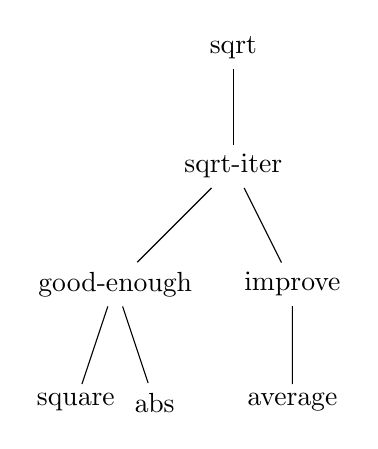
\begin{tikzpicture}[color=black]
\node {sqrt} % root
  child { node {sqrt-iter}
child[sibling distance=3cm] 
{ node{ good-enough }
child[sibling distance=1cm] 
{ node { square } }
child[sibling distance=1cm] 
{ node { abs } } }
child { node{ improve }
child { node { average } } } };
\end{tikzpicture}
\end{minipage}
\end{lstlisting}
\end{block}
\end{column}


\begin{column}{0.45\columnwidth}
\begin{block}{Result}
\begin{center}
\includegraphics[width=.9\linewidth]{pic-graphical-example-with-tikz.png}
\end{center}
\end{block}
\end{column}
\end{columns}

\note{Note
TikZ is quite verbose.
I used tikz when the exercises required drawing something.
I also redrew several figures with Tikz, as I wanted to be able to reproduce the book's narrative in my own classes (if/when I am going to give them).
Where possible, I tried to use more specific drawing tools.
Note, I did \uline{not} use TikZ for the "Functional Drawing", the so-called "Picture Language" part of SICP. 
For it I had to implements my own library, using Imagemagick.}
\end{frame}


\begin{frame}[label={sec:orgc10bdc8},fragile]{Graphical example with PlantUML. (Exercise 3.46)}
 \begin{columns}[t]
\begin{column}{0.5\columnwidth}
\lstset{numbers=none,frame=single,basicstyle=\footnotesize\ttfamily ,keywordstyle=\ttfamily,upquote=true,extendedchars=true,language=MetaPost,label= ,caption= ,captionpos=b}
\begin{lstlisting}
@startuml
skinparam monochrome true
control "  Process 1   " as p1
entity "   Mutex   " as m
control "  Process 2   "  as p2
rnote over m: false
p1 -> m: test-and-set!
p2 -> m: test-and-set!
rnote over m: set-car! cell true
rnote over m: set-car! cell true
rnote over m: true
m -> p1: false
m -> p2: false
rnote over p1: acquired
rnote over p2: acquired
@enduml
\end{lstlisting}
\end{column}


\begin{column}{0.3\columnwidth}
\begin{center}
\includegraphics[width=.9\linewidth]{exercise-3-46.png}
\end{center}
\end{column}
\end{columns}


\note{Notes
PlantUML's biggest drawback is that its syntax is ugly and fragile.
However, the team behind it is working on improving the tool, and it seems that they are learning in the process.
UML is not an as pathetic thing as it is usually thought.
Standard tools for code visualisation are certainly worth considering.
On the other hand, environment diagrams, or essentially debugging interfaces, had to be drawn with TikZ.
Which I find amusing.
Such a feature is still not possible to implement portably.}
\end{frame}

\begin{frame}[label={sec:org56ecd3f}]{How to measure progress and motivate yourself.}
\begin{columns}[t]
\begin{column}{0.45\columnwidth}
\begin{block}{Measures}
\begin{itemize}
\item Make a tree-like TODO-list
\item Count study sessions
\item Measure problem difficulty
\item Measure problem spanning days
\item Is there a way to measure creativeness?
\end{itemize}

\begin{center}
\includegraphics[height=2.5cm]{measures-breakdown.png}
\end{center}
\end{block}
\end{column}

\begin{column}{0.45\columnwidth}
\begin{block}{Motivation}
\begin{itemize}
\item Leave problems undone between sessions
\item Read problems in advance
\item Fight distractions (I failed)
\item Work chunking (pomodoro) did not work for me
\end{itemize}

\vspace{0.1cm}

\begin{center}
\includegraphics[height=2.3cm]{timer_stopwatch_flat-2442462_1280.png}
\end{center}
\end{block}
\end{column}
\end{columns}

\note{Note
\begin{itemize}
\item In high school we cross out the tasks as they appear in a problem set.
\item We feel better as things progress.
\item Measuring problem difficulty requires sequentiality.
\item Org can be compiled into a wbs-chart (not implemented)

\item Noise can be fought with headphones.
\item Pomodoro did not work because I could not fit problems in chunks reasonably.
\end{itemize}}
\end{frame}

\begin{frame}[label={sec:orgab1cd90},fragile]{Looking for help.}
 \begin{columns}[t]
\begin{column}{0.5\columnwidth}
\begin{block}{Sources}
\begin{itemize}
\item Timely help is vital
\item Many experts still use IRC (Internet Relay Chat)
\item Don't neglect everything else
\item Ignore rudeness
\item Modern messengers make it hard to mine memories
\item Videos work better at the very end of the course
\end{itemize}
\end{block}
\end{column}

\begin{column}{0.5\columnwidth}
\begin{block}{Measures}
\begin{itemize}
\item 28 Chibi-Scheme emails
\item 16 Emacs and Fortran emails
\item 20 org emails
\item 3 emails to experts
\item 16 documentation emails (+ dead link reports)
\item 2394 \texttt{\#scheme} IRC chat messages
\end{itemize}
\end{block}
\end{column}
\end{columns}

\note{Note
\begin{itemize}
\item I didn't manage to collect and reprocess memory from modern messengers.
\item The videos are like "ahh, that's what they actually meant by what they said."
\item In general, seeing "how much I have already done!" and "there is a limited amount of things to do" is a great feeling that makes you get back to work.
\item IRC is still a useful tool.
\item But the modern ones are still better to not be neglected.
\item Communication is important, and getting questions answered fast is a great thing.
\end{itemize}}
\end{frame}

\section{The Data and the Analysis.}
\label{sec:orgfd4b735}

\begin{frame}[label={sec:orgc883659},fragile]{Measured data examples.}
 \begin{block}{Session statistic}
\lstset{numbers=none,frame=single,basicstyle=\footnotesize\ttfamily ,keywordstyle=\ttfamily,upquote=true,extendedchars=true,language=elisp,label= ,caption= ,captionpos=b}
\begin{lstlisting}
[2020-05-10 Sun 14:39]-[2020-05-10 Sun 18:00] => 3:21
[2020-05-09 Sat 19:13]-[2020-05-09 Sat 22:13] => 3:00
[2020-05-09 Sat 09:34]-[2020-05-09 Sat 14:34] => 5:00
...
\end{lstlisting}
\end{block}

\begin{block}{Problem statistic.}
\lstset{numbers=none,frame=single,basicstyle=\footnotesize\ttfamily ,keywordstyle=\ttfamily,upquote=true,extendedchars=true,language=elisp,label= ,caption= ,captionpos=b}
\begin{lstlisting}
Figure 1.1 Tree with the values of subcombinations
[2019-08-20 Tue 14:35]
Exercise 1.1 Interpreter result
[2019-08-20 Tue 14:23]
Exercise 1.2 Prefix form
[2019-08-20 Tue 14:25]
...
\end{lstlisting}
\end{block}

\note{Note
Problem statistic is indicative.
I first solved the Exercises 1.1 and 1.2, and then turned to the Figure 1.1.
But it is displayed earlier, because it is earlier in the book.

Solving problems has a little bit of robustness to non-sequentiality.
In general, SICP tries to enforce sequentiality by making problems depend on one another, and this gives the noweb-like features of SICP a great value.

Having time tracking data in a machine-accessible format made it possible to do the analysis.}
\end{frame}

\begin{frame}[label={sec:org93ff09a},fragile]{Data analysis with Emacs Lisp.}
 \begin{columns}[t]
\begin{column}{0.45\columnwidth}
\begin{block}{Emacs Lisp for analysis}
\lstset{numbers=none,frame=single,basicstyle=\footnotesize\ttfamily ,keywordstyle=\ttfamily,upquote=true,extendedchars=true,language=elisp,label= ,caption= ,captionpos=b,basicstyle=\scriptsize\ttfamily,upquote=true,numbers=left,emph={cl-labels,seq-concatenate},emphstyle=\color{red},frame=leftline}
\begin{lstlisting}
(require 'org-element)
(cl-labels (
 ; lexical-defun
(decorate-orgtable (tbl)
  (seq-concatenate
   'string
   "("
"| Exercise| Days| Sessions| Minutes|" 
(char-to-string ?\n)
"|- + - + - + - |"
(format-orgtable tbl)
")")
)
; lexical-defun
(format-orgtable (list-of-lists) ...
\end{lstlisting}
\end{block}
\end{column}

\begin{column}{0.5\columnwidth}
\begin{block}{Problem summaries}
\vspace{0.26cm}
\scriptsize
\begin{supertabular}{|l|p{3.0cm}|p{0.6cm}|p{0.6cm}|p{0.6cm}|}
\hline
No & Exercise Name & Days Spent & Spans Sessions & Minutes Spent\\
\hline
1 & Exercise 1.1 Interpreter result & 1.211 & 2 & 459\\
2 & Exercise 1.2 Prefix form & 0.001 & 1 & 2\\
3 & Figure 1.1 Tree representation & 0.007 & 1 & 10\\
4 & Exercise 1.4 Compound expressions & 0.003 & 1 & 4\\
5 & Exercise 1.5 Ben's test & 0.008 & 1 & 11\\
6 & Exercise 1.6 If is a special form & 0.969 & 2 & 118\\
7 & Exercise 1.7 Good enough? & 0.949 & 3 & 436\\
\end{supertabular}
\end{block}
\end{column}
\end{columns}



\note{Note
\begin{itemize}
\item This is called ``Reproducible Research''.
\item seq-* functions help elisp be like scheme.
\item cl-labels are like lexical defuns.
\item The ten problems on the right are the example of the table that the code generates, and the table can be further analyzed by Emacs Lisp.
\item The three measures are "raw time", "wall clock time" and "total days in memory".
\item They all are not totally dependent.
\item It is possible to offload some thinking into the unconscious.
\item It is easier to return to the work when you have something undone.
\item Problems were never ended at the same time as sessions.
\end{itemize}}
\end{frame}


\begin{frame}[label={sec:org0761ff9},shrink=30]{Data demonstration.}
\begin{columns}[t]
\begin{column}{0.5\columnwidth}
\begin{center}
\includegraphics[width=.9\linewidth]{experience-report-days.png}
\end{center}
\begin{center}
\includegraphics[width=.9\linewidth]{experience-report-study-sessions.png}
\end{center}
\end{column}
\begin{column}{0.5\columnwidth}
\begin{center}
\includegraphics[width=.9\linewidth]{experience-report-minutes-per-problem.png}
\end{center}
\begin{center}
\includegraphics[width=.9\linewidth]{experience-report-hardness-histogram-logarithmic.png}
\end{center}
\end{column}
\end{columns}

\note{Notes
Not really readable graphs depict the distribution of the three measures of the dataset.
Problems that take more days than sessions are essentially the days when I needed a holiday.
But students also have holidays.
Why exactly the problem set obeys a log-normal distribution?
The two most difficult problems take most of the time.
To me it would mean that those have to be broken into smaller bits.
Even though is says "translate scheme to a low-level language line by line", the runtime support is huge, and not very well explained in SICP.
Input-output is not explained at all.
This is not what students usually do in the university, but perhaps it is not such a bad thing.}
\end{frame}


\begin{frame}[label={sec:orgbf134b6},fragile]{Statistics and ten hardest problems.}
 \begin{columns}[t]
\begin{column}{0.5\columnwidth}
\scriptsize
\begin{itemize}
\item \alert{729} hours total work duration.
\item \alert{2.184} hours mean time spent on solving one problem.
\item \alert{0.96} hours was required for the dataset median problem.
\item \alert{94.73} hours for the hardest problem: writing a Scheme interpreter in a low-level language.
\item \alert{652} study sessions.
\item \alert{1.79} study sessions per problem on average.
\item \alert{1} median number of study sessions required to solve a single problem.
\item \alert{>78000}-lines long .org file (\alert{>2.6} megabytes) (5300 pages in a PDF).
\item \alert{13} problems were solved out of order.
\end{itemize}
\end{column}

\begin{column}{0.6\columnwidth}
\vspace{-0.15cm}
\scriptsize
\begin{center}
\begin{supertabular}{p{4cm}|p{0.7cm}|p{0.5cm}|p{0.5cm}}
Exercise & Days & Sessions & Minutes\\
\hline
Exercise 2.46 \texttt{make-vect}. & 2.578 & 5 & 535\\
Exercise 4.78 Non-deterministic queries. & 0.867 & 6 & 602\\
Exercise 3.28 Primitive or-gate. & 1.316 & 2 & 783\\
Exercise 4.79 Prolog environments. & 4.285 & 5 & 940\\
Exercise 3.9 Environment structures. & 21.03 & 10 & 1100\\
Exercise 4.77 Lazy queries. & 4.129 & 9 & 1214\\
Exercise 4.5 \texttt{cond} with arrow. & 12.765 & 7 & 1252\\
Exercise 5.52 Making a compiler for Scheme. & 22.975 & 13 & 2359\\
Exercise 2.92 Add, mul for different variables. & 4.556 & 11 & 2404\\
Exercise 5.51 EC-evaluator in low-level language. & 28.962 & 33 & 5684\\
\end{supertabular}
\end{center}
\end{column}
\end{columns}

\note{Note
\begin{itemize}
\item make-vect -- writing the whole picture language
\item non-deterministic -- whole rewrite
\item primitive or-gate -- assemble a simulator
\item prolog-env -- open-ended
\item environment structures -- TikZ
\item lazy-queries -- a large architectural piece
\item cond with arrow -- assemble a metacircular evaluator
\item scheme compiler -- huge
\item add+mul different variables -- huge work with normalization
\item ec-evaluator -- learning fortran

\item Three working months (>700 hours)
\end{itemize}}
\end{frame}

\section{Results and Conclusion.}
\label{sec:orgff97947}

\begin{frame}[label={sec:org07dd519},fragile,squeeze]{By-products of the work.}
 \begin{columns}
\begin{column}{0.6\columnwidth}
\begin{itemize}
\item \texttt{STk} \alert{resurrected}, thanks to Eric Gallesio
\item \texttt{psd} \alert{resurrected} on github, thanks to Pertti Kellomaki
\item \alert{4 bugs} in \texttt{gfortran} fixed (1 critical)
\item \alert{2 bugs} in \texttt{Chibi-Scheme} fixed
\item a few small \alert{bugs} in \texttt{Emacs} found/mitigated
\item \alert{SRFI-203} (Picture Language) -- draft
\item ``complete'' solution to SICP in pdf
\item Scheme Workshop \alert{report}
\item \alert{SRFI-2??} (SICP prerequisites) -- pre-draft
\item Yet another scheme \alert{interpreter} (\texttt{schemetran})
\end{itemize}

(SRFIs are Scheme Requests for Implementation.)
\end{column}

\begin{column}{0.4\columnwidth}
\begin{center}
\includegraphics[width=.9\linewidth]{by-products-lambda-from-wiki.png}
\end{center}
\end{column}
\end{columns}

\note{Note
This project gave birth to a healthy amount of by-products.
The most universally useful is probably the bug fix in gnu fortran, which I used for the last two exercises.
Twice I got a remark from old software writers that "software never dies".
I didn't manage to port PSD to a modern Emacs, but this probably can be done eventually.

Let's talk about portability.
Even though SICP is believed to be a book about scheme, it is still not possible to finish it with a scheme system supporting only the base standard, even if it is r7rs.
The critical points are multi-threading, randomness, and most prominently, graphics.
I think that this is a drawback, and should be addressed.
I already submitted an srfi on the most unportable part.
The second, one on the parts that are implementable with the help of other SRFIs, is in the plans.}
\end{frame}

\begin{frame}[label={sec:org5deabd9}]{Applications and Further Work.}
\begin{columns}[t]
\begin{column}{0.45\columnwidth}
\begin{block}{Applications}
\begin{description}
\item[{Teachers}] monitor dropout
\item[{Teachers}] make marking simpler
\item[{Students}] make portfolios
\item[{Students}] monitor work
\item[{Designers}] make coursework templates
\item[{Designers}] get feedback
\end{description}
\end{block}
\end{column}

\begin{column}{0.45\columnwidth}
\begin{block}{\alert{We Need More Data!}}
\begin{itemize}
\item Get more data points for SICP!
\item Behavioural analysis of the existing data.
\item Measure other course work!
\item Profile-guided optimisation.
\item Social/cloud service.
\item Effort tracking? (e.g. window switching)
\end{itemize}
\end{block}
\end{column}
\end{columns}

\note{Notes
On this slide I want to once again restate that for me this project can be seen as a model according to which university coursework could be considered.
Having an established notion of a "standard coursework" would allow to calibrate one's own perception.
Am I late or ahead?
Do I have enough time scheduled for the work?
Where am I in the process.
How do I recall the learned topics in the future?

Same things apply to the teachers, only regarding their students.
In addition, it may be mildly nice for the teachers to have an example of a "well-done coursework" that can be shown to the students.
Obviously, a single-point estimate is not very good.
Teachers have a power over their student, at least in the form of exposing them to the existence of this report.}
\end{frame}

\begin{frame}[label={sec:orgc1a2302}]{Review.}
\begin{columns}
\begin{column}{0.4\columnwidth}
\begin{center}
\includegraphics[width=.9\linewidth]{SICP_cover.png}
\end{center}
\end{column}

\begin{column}{0.5\columnwidth}
\begin{itemize}
\item A full year of work. (Three months of raw time.)
\item Fitting SICP into one semester seems hard.
\item Almost no superfluous topics.
\item Several subjects are omitted.
\item Many by-products.
\item Lots of software is buggy.
\item Learning requires audacity.
\item Computer-assisted learning goes smoother.
\end{itemize}
\end{column}
\end{columns}

\note{Notes
This course is hard.
Can I say that it is needlessly hard?
It certainly requires spending a lot of time on learning things that are not even mentioned in the book.
In fact, the book looks more like a companion to the MIT course than a standalone work.
I hope that the SRFIs and this Report can compensate for that a little bit, and help those trying to solve SICP in the future by sawing off the sharp corners.
All of this took roughly one year, including the Report and the SRFIs.
Learning while being employed is certainly possible, but hard.
Computing models presented in SICP seem not obsolete.
?}
\end{frame}

\begin{frame}[label={sec:orgfc2f970},fragile]{Credits.}
 \begin{columns}[t]
\begin{column}{0.5\columnwidth}
\begin{block}{Contacts}
\begin{itemize}
\item \url{http://gitlab.com/Lockywolf}
\item \url{http://lockywolf.wordpress.com}
\item \texttt{lockywolf at gmail.com}
\item \url{https://t.me/unobvious}
\item \url{http://lockywolf.net}
\item \href{https://paypal.me/independentresearch}{https://paypal.me/independentresearch}
\end{itemize}
\end{block}
\end{column}

\begin{column}{0.5\columnwidth}
\begin{block}{Thank you}
\begin{itemize}
\item John Cowan
\item Alex Shinn
\item Eli Zaretskii
\item Patrick Volkerding
\item evets @ \url{stackoverflow}
\item \texttt{irc.freenode.net/\#scheme} contributors
\item all my friends and relatives
\end{itemize}
\end{block}
\end{column}
\end{columns}

\note{Notes
I want to say thank you to the \texttt{\#scheme} freenode channel users.
Personal thank you to the people responsible for the scheme standard development, for the implementation development, for Emacs development, Fortran developers, Slackware developers.}
\end{frame}
\end{document}